\section{Analysis of results}
In this project, multi-node parallelization of the existing serial code for simulation of conservation laws have been performed. Multi-node parallelization enables the program to use the capabilities of a server consists of several nodes and each node having various computing units connected with fast interconnects such as {\ttfamily InfiniBand}. Each node also have its own memory hence in order to get access to other process's memory we need to exclusively communicate the information that we want the other process to have access and there comes {\ttfamily MPI} into the picture.

The parallel code has been tested by running two problems: \textbf{Kelvin-Helmholtz instability} and \textbf{isentropic Euler vortex}. The scaling tests for both of these problems have been performed and results are shown.
\subsection{Speedup calculation}
The speed up results have been shown for the parallel code. These speedup results are in comparison to serial code execution time which is essentially running the parallel code with total number of process as 1. Formula used for calculation speedup is
\begin{equation*}
    \text{Speedup} = \frac{\text{Execution time with 1 process}}{\text{Execution time with N processes}}
\end{equation*}
For \textbf{Kelvin-Helmholtz instability}, \\
Execution time with 1 process: 68230.47 seconds\footnote[3]{All the data has been collected on Dual Intel(R) Xeon(R) Gold 6148 CPU @ 2.40GHz}\\
Execution time with 16 process: 5157.72 seconds
\begin{equation*}
    \text{Speedup} = \frac{68230.47}{5157.72} = 13.23~~\text{times}
\end{equation*}
\linebreak
For \textbf{isentropic Euler vortex},\\
Execution time with 1 processes: \footnotemark[3] \\
Execution time with 16 processes: 14904 seconds
\begin{equation*}
    \text{Speedup} = \frac{}{14904} = ~~\text{times}
\end{equation*}
\vspace{10pt}
\subsection{Efficiency calculation}
The efficiency of a parallel code is a measure of how effectively a parallel program is able to utilize the available computational resources compared to its sequential counterpart. It is calculated by:
\begin{equation*}
    \text{Efficiency} = \frac{\text{Speedup}}{\text{Number of processors}} \times 100 \%
\end{equation*}
For \textbf{Kelvin-Helmholtz instability},\\
Speedup = 13.23\\
Total number of processes = 16
\begin{equation*}
    \text{Efficiency} = \frac{13.23}{16} \times 100 \% = 82.7 \%   
\end{equation*}
\begin{figure*}[!ht]
    \centering
    \begin{minipage}{0.5\textwidth}
        \centering
        
\includegraphics[width=0.9\linewidth]{attachments/kelvin_8.0000.png}
        \caption*{(a)}
    \end{minipage}%
    \begin{minipage}{0.5\textwidth}
        \centering
        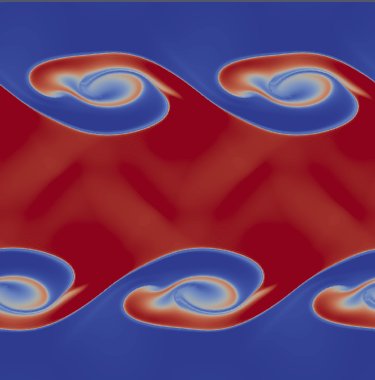
\includegraphics[width=0.9\linewidth]{attachments/kelvin_8.0264.png}
        \caption*{(b)}
    \end{minipage}
    \caption{Kelvin-Helmholtz instability at $t = 3$ using polynomial degree $N = 4$, (a) Initial condition, (b) density plot}
\end{figure*}

\hspace{-18pt}For \textbf{isentropic Euler vortex},\\
Speedup = \\
Total number of processes = 16
\begin{equation*}
    \text{Efficiency} = \frac{}{16} \times 100 \% =  \%   
\end{equation*}
\begin{figure*}[!ht]
    \centering
    \begin{minipage}{0.5\textwidth}
        \centering
        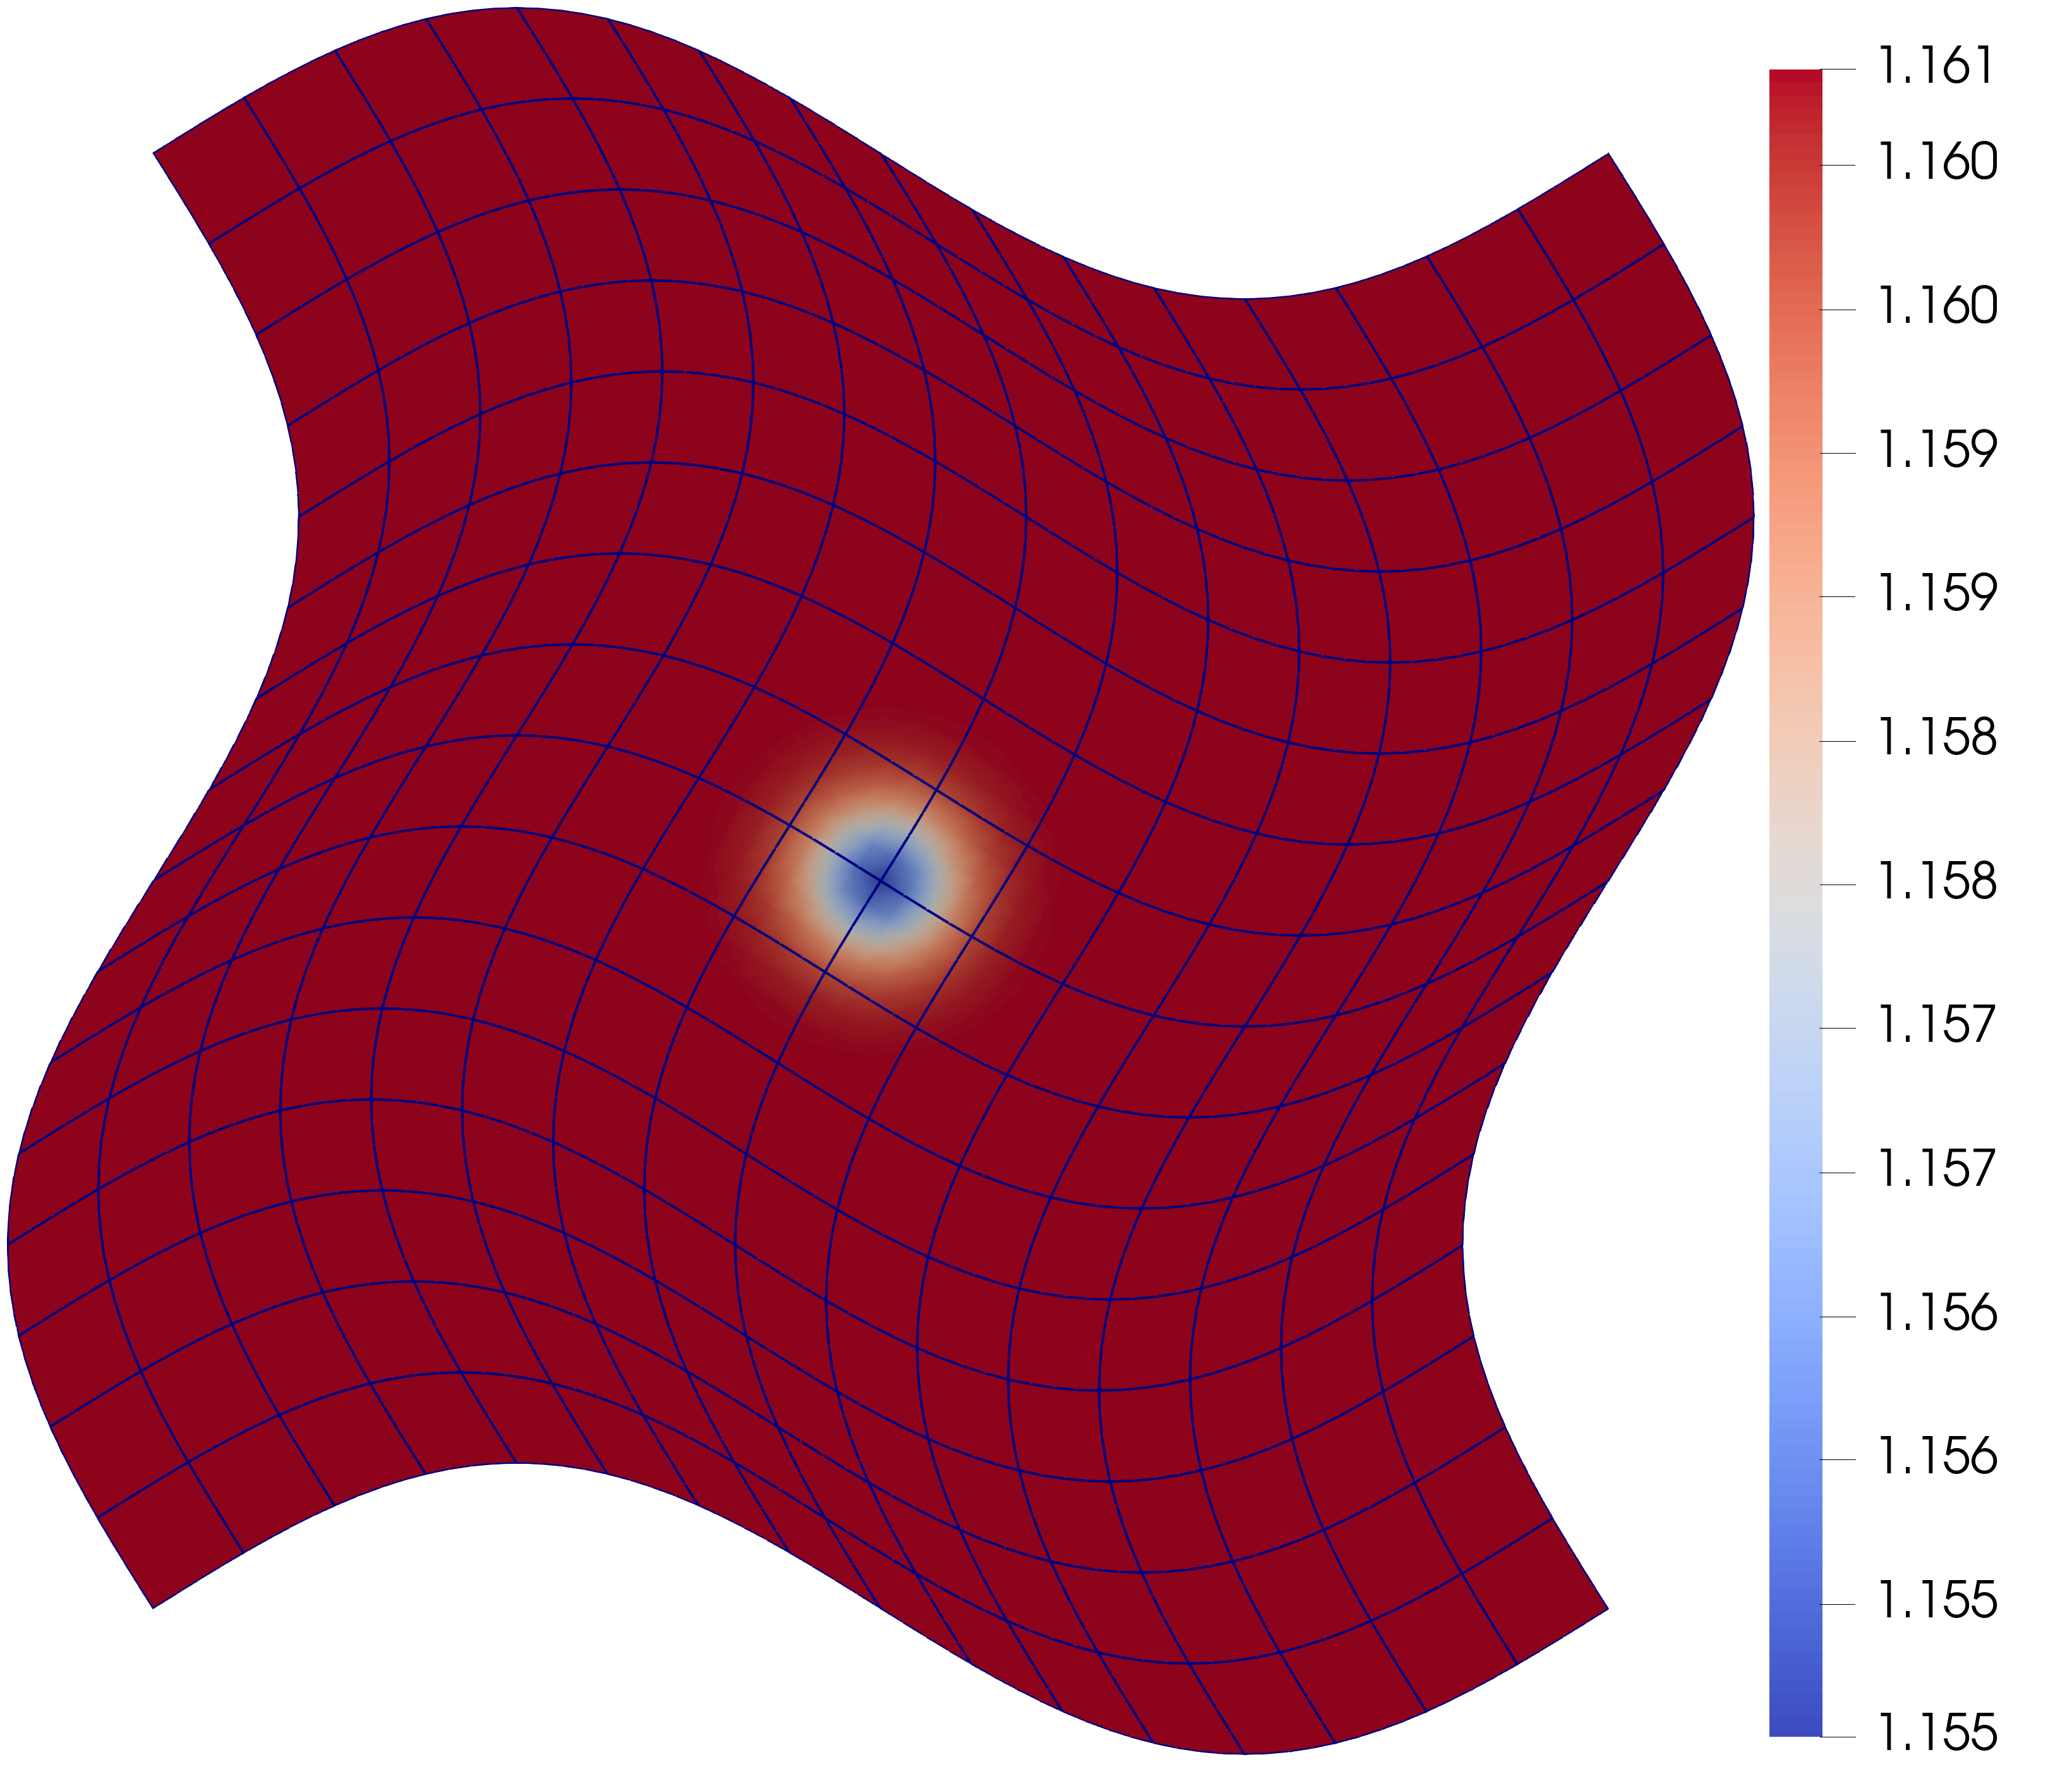
\includegraphics[width=0.9\linewidth]{attachments/isentropic_arpit.png}
        \caption*{(a)}
    \end{minipage}%
    \begin{minipage}{0.5\textwidth}
        \centering
        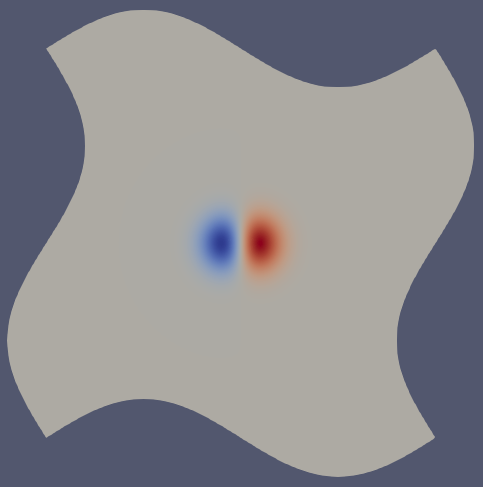
\includegraphics[width=0.9\linewidth]{attachments/solution_068877_vx.png}
        \caption*{(b)}
    \end{minipage}
    \caption{Isentropic vortex using polynomial degree $N = 4$, (a) density plot, (b) velocity in x direction}
\end{figure*}
\section{Scaling test} \label{st}
The numbers in speedup and efficiency that we got in results shows a promising hope for the problems of real world involving complex CFD simulations, big data etc., to be simulated using multi-node environment. These results can be improved further with better optimization techniques and utilising the features of modern hardware such as vector processors etc. 


\begin{center}
    \rule{3cm}{1pt}
\end{center}